\documentclass[conference]{IEEEtran}
%\documentclass[draftcls]{IEEEtran}
%\documentclass{article} \usepackage{IEEEtrantools}

\usepackage{cite}
\usepackage{url}
\usepackage{graphicx}
\usepackage[caption=false,font=footnotesize]{subfig}
\usepackage{color}
\usepackage{amsmath}
\usepackage{amsfonts}
\usepackage{bbm}
\usepackage{algorithmic}

\graphicspath{{figures/}}
%%% MACROS FOR MATHEMATICAL NOTATION IN COMPOSITE PROPOSAL PAPER %%%

% Functions and operators
\newcommand{\half}{\frac{1}{2}}                                 % Half
\newcommand{\expect}[1]{\mathbb{E}_{#1}}                        % Expectation
\newcommand{\variance}[1]{\mathbb{V}_{#1}}                      % Variance
\DeclareMathOperator{\trace}{Tr}                                % Trace
\newcommand{\magdet}[1]{\left| #1 \right|}         % Magnitude of the determinant
\newcommand{\indic}[1]{\mathbbm{1}_{#1}}                        % Indicator function
\newcommand{\normal}[3]{\mathcal{N}\left(#1\left|#2,#3\right.\right)}       % Normal density
\newcommand{\gammaden}[3]{\mathcal{\Gamma}\left(#1|#2,#3\right)}% Gamma density
\newcommand{\studentt}[4]{\mathcal{ST}\left(#1|#2,#3,#4\right)} % Student-t density
\newcommand{\bigo}[1]{\mathcal{O}\left({#1}\right)}             % Big O
\newcommand{\mhaccept}{\alpha}                                  % Metropolis-Hastings acceptance probability

% Basics
\newcommand{\rt}{t}                             % Real time
\newcommand{\pt}{\lambda}                       % Pseudo-time
\newcommand{\dpt}{\delta\lambda}                % A little bit of pseudo-time
\newcommand{\ls}[1]{x_{#1}}                     % Latent state
\newcommand{\ob}[1]{y_{#1}}                     % Observation
\newcommand{\mix}[1]{\xi_{#1}}                  % Mixing auxiliary variable
\newcommand{\els}[1]{u_{#1}}                    % Extra latent state

% Particle shizzle
\newcommand{\pss}[2][]{^{(#2)#1}}               % Particle superscript
\newcommand{\pw}[1]{w_{#1}}                     % Particle weight
\newcommand{\predpw}[1]{\hat{w}_{#1}}           % Predictive particle weight
\newcommand{\npw}[1]{\bar{w}_{#1}}              % Normalised particle weight
\newcommand{\naw}[1]{\bar{v}_{#1}}              % Normalised auxiliary weight
\newcommand{\anc}[1]{a_{#1}}                    % Particle ancestor

% Densities
\newcommand{\transden}{f}                       % Transition density
\newcommand{\obsden}{g}                         % Observation density
\newcommand{\impden}{q}                         % Importance density
\newcommand{\partden}{\eta}                     % Unweighted particle distribution
\newcommand{\artden}{\rho}                      % Artificial conditional density
\newcommand{\oiden}[1]{\pi_{#1}}                % Optimal importance density
\newcommand{\approxoiden}[2]{\hat{\pi}_{#1|#2}} % Approximation of the optimal importance density
\newcommand{\augfiltden}[1]{\tilde{\pi}_{#1}}   % Augmented filtering density
\newcommand{\oinorm}[1]{K_{#1}}                 % Normalising constant for the optimal importance density
\newcommand{\augfiltnorm}[1]{\tilde{K}_{#1}}    % Normalising constant for the augmented filtering density

% Numbers
\newcommand{\numpart}{N_F}                      % Number of filter particles
\newcommand{\ess}[1]{N_{E,#1}}                  % Effective sample size

% Models
\newcommand{\transfun}{\phi}                    % Transition function
\newcommand{\obsfun}{h}                         % Observation function
\newcommand{\transcov}{Q}                       % Transition covariance
\newcommand{\obscov}{R}                         % Observation covariance
\newcommand{\transmat}{F}                       % Linear transition matrix
\newcommand{\obsmat}{H}                         % Linear observation matrix
\newcommand{\transmean}{m}                      % Mean of the transition density (i.e. f(x_{t-1}))
\newcommand{\dof}{\nu}                          % Degrees of freedom of something student-t-ish

% Linear Gaussian things
\newcommand{\lgoimean}[1]{\mu_{#1}}             % Linear Gaussian optimal importance density mean
\newcommand{\lgoicov}[1]{\Sigma_{#1}}           % Linear Gaussian optimal importance density covariance
\newcommand{\stdnorm}[1]{z_{#1}}                % Standard normal R.V.

% Gaussian Transformation
\newcommand{\lgdecayfunc}{a}                    % Linear Gaussian decay function for OID transformation
\newcommand{\lgexpsf}{\gamma}                   % Linear Gaussian exponential scale factor for OID transformation
\newcommand{\lgupdmeanmat}[1]{\Gamma_{#1}}      % Mean mapping matrix for the OID transformation
\newcommand{\lgupdcov}[1]{\Omega_{#1}}          % Covariance matrix for the OID transformation
\newcommand{\lginfbm}[1]{\epsilon_{#1}}         % Brownian motion for the infinitesimal form of the OID transformation

% Linear Gaussian approximations
%\newcommand{\lgoimeanapprox}[2]{\hat{\mu}_{#1}(#2)}     % Mean of the Gaussian approximation to the OID at time #1 and state #2
%\newcommand{\lgoicovapprox}[2]{\hat{\Sigma}_{#1}(#2)}   % Covariance of the Gaussian approximation to the OID at time #1 and state #2
\newcommand{\lgoimeanapprox}[2]{\hat{\mu}_{#1|#2}}      % Mean of the Gaussian approximation to the OID at time #1 and state #2
\newcommand{\lgoicovapprox}[2]{\hat{\Sigma}_{#1|#2}}    % Covariance of the Gaussian approximation to the OID at time #1 and state #2
\newcommand{\obsmatapprox}[1]{\hat{\obsmat}_{#1}}       % Linear observation matrix formed by differentiation of the observation function
\newcommand{\transmeanapprox}[1]{\hat{\transmean}_{#1}} % Approximate transition mean
\newcommand{\transcovapprox}[1]{\hat{\transcov}_{#1}}   % Approximate transition covariance
\newcommand{\obapprox}[1]{\hat{y}_{#1}}                 % Approximate observation mean
\newcommand{\obscovapprox}[1]{\hat{\obscov}_{#1}}       % Approximate observation covariance
\newcommand{\lsfixed}{\ls{}^*}                          % Latent state around which we linearise
\newcommand{\logtrans}{L}                               % Log of the transition density
\newcommand{\logobs}{M}                                 % Log of the observation density

% State evolution SDE
\newcommand{\oudrift}[1]{A_{#1}}                % General O-U process drift term
\newcommand{\oudiffuse}[1]{B_{#1}}              % General O-U process diffusion term
\newcommand{\sdedrift}[1]{\zeta_{#1}}           % Drift
\newcommand{\lserror}[2]{e_{#1|#2}}             % State error due to finite sampling

% Particle flow
\newcommand{\flowbm}[1]{\epsilon_{#1}}          % Particle flow Brownian motion
\newcommand{\flowdrift}[1]{\zeta_{#1}}          % Particle flow drift
\newcommand{\flowdiffuse}[1]{\eta_{#1}}         % Particle flow diffusion
\newcommand{\flowcov}[1]{D_{#1}}                % Particle flow "Covariance" matrix
\newcommand{\flowtd}{\alpha}                    % Flow dervation transition density
\newcommand{\flowod}{\beta}                     % Flow derivation observation density

% Simulation models - tracking
\newcommand{\pos}[1]{p_{#1}}           % Position
\newcommand{\vel}[1]{v_{#1}}           % Velocity
\newcommand{\bng}[1]{\theta_{#1}}               % Bearing
\newcommand{\rng}[1]{r_{#1}}                    % Range
\newcommand{\hei}[1]{h_{#1}}                    % Height
\newcommand{\rngrt}[1]{s_{#1}}                  % Range rate
\newcommand{\terrain}{T}                        % Terrain height

% Simulation models - heartbeats
\newcommand{\amp}[1]{A_{#1}}                    % Amplitude
\newcommand{\wid}[1]{W_{#1}}                    % Width
\newcommand{\del}[1]{\tau_{#1}}                 % Delay
\newcommand{\freq}[1]{\omega_{#1}}              % Width
\newcommand{\pha}[1]{\psi_{#1}}                 % Phase
\newcommand{\bias}[1]{B_{#1}}                   % Bias


\hyphenation{}

\newenvironment{meta}[0]{\color{red} \em}{}

\begin{document}

\title{Particle Filtering with Composite Gaussian Approximations to the Optimal Importance Density}
\author{\IEEEauthorblockN{Pete Bunch}
\IEEEauthorblockA{Signal Processing and Communications Lab.\\
Cambridge University Engineering Dept.\\
Cambridge, UK,\\
Email: pb404@cam.ac.uk}
%\and
%\IEEEauthorblockN{Simon Godsill}
%\IEEEauthorblockA{Signal Processing and Communications Lab.\\
%Cambridge University Engineering Dept.\\
%Cambridge, UK,\\
%Email: sjg30@cam.ac.uk}
}

\maketitle

\begin{abstract}
A new algorithm, the composite proposal particle filter, is introduced. The performance of a standard particle filter is highly dependent on the choice of importance density used to propagate the particles through time. The conditional posterior state density is the optimal choice, but this can rarely be calculated analytically or sampled from exactly. Practical particle filters rely forming approximations to the optimal importance density, frequently using Gaussian distributions, but these are not always effective on highly nonlinear models. The composite proposal method introduces the effect of each observation gradually and incrementally modifies the particle states so as to achieve an improved approximation to the optimal importance distribution.
\end{abstract}


\IEEEpeerreviewmaketitle



\section{Introduction}

Particle filters are an established class of algorithms for approximating the Bayesian filtering distribution of a latent state in a sequential model. (See \cite{Cappe2007,Doucet2009}.) Their mechanism is to propagate a set of weighted samples, or ``particles'', through time, distributed roughly according to the desired filtering distribution. The particles are propagated by importance sampling; a new state is sampled from an importance density and assigned a weight proportional to the ratio of the filtering and importance densities.

The efficacy of a particle filter depends substantially on the choice of importance density. If it is well matched to the filtering density then the resulting particles will have even weights, and the filter works well. On the other hand, if there is a mismatch between the densities, the population is likely to be dominated by a small proportion of particles with high weights, and the filter works poorly.

The optimal choice for the importance density --- in the sense of minimising the weight variance --- is the conditional posterior density of the state. However, this can rarely be sampled from or evaluated exactly. Instead, it is common to use approximations, for example by choosing some appropriately adapted Gaussian density \cite{Doucet2000a}. For many mildly nonlinear models such an approximation has proven most effective, but as the nonlinearity and dimensionality increase, and the modes of the optimal importance density become less and less Gaussian, performance becomes worse.

In this paper, we introduce a new mechanism for conducting the importance sampling steps in a particle filter. The effect of each new observation is introduced gradually, and a new state is proposed for each incremental step using a local Gaussian approximation. Since each final particle state is reached via series of intermediate steps, we name this algorithm the composite proposal particle filter (CPPF). By using small steps and adapting the approximations to the current state, a more accurate approximation to the optimal importance density is achieved, and the resulting filter proves more effective than competitors using a single Gaussian as the importance density.

The concept of introducing the likelihood progressively is not original. It has been used for estimation of normalising constants \cite{Gelman1998}, for assumed density filtering \cite{Hanebeck2003a,Hanebeck2012,Hagmar2011}, and in annealed particle filters \cite{Godsill2001b,Neal2001,Gall2007,Deutscher2000}. Annealed particle filters rely on the use of intermediate particle selection steps to rejuvenate the population, introducing dependency between the particles in the process. In contrast, the CPPF simply uses the progressive framework to construct an improved approximation to the optimal importance density. Particle state proposals are still entirely independent.



\section{Particle Filtering}

We consider a standard discrete-time HMM in which the transition, observation and prior models have closed-form densities,
%
\begin{IEEEeqnarray}{rCl}
 \ls{\rt} & \sim & \transden(\ls{\rt} | \ls{\rt-1}) \label{eq:td} \\
 \ob{\rt} & \sim & \obsden(\ob{\rt} | \ls{\rt})   \label{eq:od} \\
 \ls{1} & \sim & p(\ls{1})                  \label{eq:pd}      ,
\end{IEEEeqnarray}
%
where the random variable $\ls{\rt}$ is the hidden state of a system at time $\rt$, and $\ob{\rt}$ is an incomplete, noisy observation. We assume here that the transition, observation and prior densities may be evaluated and that the prior and transition densities may be sampled. A particle filter is used to estimate recursively distributions over the path of the state variables, $\ls{1:\rt}=\{\ls{1}, \dots, \ls{\rt}\}$. Densities are approximated by a sum of weighted probability masses located at a discrete set of states,
%
\begin{IEEEeqnarray}{rCl}
 p(\ls{1:\rt} | \ob{1:k}) & = & \sum_i \npw{\rt}\pss{i} \delta_{\ls{1:\rt}\pss{i}}(\ls{1:\rt})     ,
\end{IEEEeqnarray}
%
where $\delta_{\ls{1:\rt}\pss{i}}(\ls{1:\rt})$ denotes a unit probability mass at the point $\ls{1:\rt}\pss{i}$.

The particle filter recursion may be separated into two stages --- prediction and update --- which produce approximations to the predictive, $p(\ls{1:\rt} | \ob{1:\rt-1})$, and filtering, $p(\ls{1:\rt} | \ob{1:\rt})$, densities respectively.

At time $\rt$, the prediction stage begins with selection (resampling) of a parent from amongst the $\rt-1$ particles; an index, $\anc{j}$, is chosen with probability $\npw{t-1}\pss{j}$. (This is the most basic algorithm, in which selection is not optional and no ``auxiliary filtering'' is used.) Next, a new state $\ls{\rt}\pss{j}$ is sampled from an importance density, $\impden(\ls{\rt} | \ls{\rt-1}\pss{\anc{j}}, \ob{\rt})$, and concatenated to the parent path to form the new particle,
%
\begin{IEEEeqnarray}{rCl}
 \ls{1:\rt}\pss{j} \leftarrow \left\{ \ls{1:\rt-1}\pss{\anc{j}},  \ls{\rt}\pss{j} \right\}     .
\end{IEEEeqnarray}
%
Finally, an importance weight is assigned to the particle to account for the discrepancy between importance and target distributions,
%
\begin{IEEEeqnarray}{rCl}
 \predpw{\rt}\pss{j} & = & \frac{ p(\ls{1:\rt}\pss{j} | \ob{1:\rt-1}) }{ p(\ls{1:\rt-1}\pss{\anc{j}} | \ob{1:\rt-1}) \impden(\ls{\rt}\pss{j} | \ls{\rt-1}\pss{\anc{j}}, \ob{\rt}) } \nonumber \\
 & \propto & \frac{ \transden(\ls{\rt}\pss{j} | \ls{\rt-1}\pss{\anc{j}}) }{ \impden(\ls{\rt}\pss{j} | \ls{\rt-1}\pss{\anc{j}}, \ob{\rt}) }     .
\end{IEEEeqnarray}

In the update stage, the same set of particles is used to approximate the filtering distribution. These are distributed according to $\partden(\ls{1:\rt} | \ob{1:\rt})$, where,
%
\begin{IEEEeqnarray}{rCl}
 p(\ls{1:\rt}\pss{j} | \ob{1:\rt-1}) & \propto & \predpw{\rt}\pss{j} \partden(\ls{1:\rt}\pss{j} | \ob{1:\rt}) \nonumber      .
\end{IEEEeqnarray}
%
A new importance weight is required to account for the discrepancy,
%
\begin{IEEEeqnarray}{rCl}
 \pw{\rt}\pss{j} & =       & \frac{ p(\ls{1:\rt}\pss{j} | \ob{1:\rt}) }{ \partden(\ls{1:\rt}\pss{j} | \ob{1:\rt}) } \nonumber \\
                 & \propto & \predpw{\rt}\pss{j} \times \obsden(\ob{\rt} | \ls{\rt}\pss{j} )      .
\end{IEEEeqnarray}
%
Finally, the weights are normalised,
%
\begin{IEEEeqnarray}{rCl}
 \npw{\rt} & = & \pw{\rt}\pss{j} \Big/ \sum_i \pw{\rt}\pss{i}      .
\end{IEEEeqnarray}

If the transition density is used as the importance density then the resulting algorithm is the ``bootstrap filter'' of \cite{Gordon1993}. The optimal importance density (OID) is the conditional state posterior,
%
\begin{IEEEeqnarray}{rCl}
 \impden(\ls{\rt} | \ls{\rt-1}\pss{\anc{j}}, \ob{\rt}) & = & p(\ls{\rt} | \ls{\rt-1}\pss{\anc{j}}, \ob{\rt}) \label{eq:OID}      .
\end{IEEEeqnarray}
%
However, the normalising constant for this density is an integral which cannot be calculated analytically except in a few special cases. For other models, it is common to use Gaussian approximations of \eqref{eq:OID} based on either linearisation or the unscented transform \cite{Doucet2000a,Merwe2000}.  These work well when the OID is unimodal, and the observation nonlinearity is weak, but can otherwise perform very poorly.



\section{Composite Proposals}

The composite proposal method is a procedure for sampling approximately from the OID by introducing the likelihood progressively and making a series of local Gaussian approximations. In order to achieve this, an auxiliary variable $\pt \in [0,1]$ is used. Intuitively, this is a stretch of ``pseudo-time'' between the predictive and filtering densities, which we link via a continuous sequence of densities,
%
\begin{IEEEeqnarray}{rCl}
 \augfiltden{\rt,\pt}(\ls{1:\rt-1}, \ls{\rt,\pt}) & = & \frac{ \obsden(\ob{\rt} | \ls{\rt,\pt})^{\pt} \transden(\ls{\rt,\pt} | \ls{\rt-1}) p(\ls{1:\rt-1}|\ob{1:\rt-1}) }{ \int \obsden(\ob{\rt} | \ls{\rt,\pt})^{\pt} p(\ls{\rt,\pt} | \ob{1:\rt-1}) d\ls{\rt,\pt} } \IEEEeqnarraynumspace   \label{eq:filtering_sequence}      ,
\end{IEEEeqnarray}
%
in which $\ls{\rt,\pt}$ is defined as the state at time $\rt$ and pseudo-time $\pt$. This filtering sequence includes the predictive density when $\pt=0$ and the desired filtering density when $\pt=1$.

State updates are derived by considering a related sequence of optimal importance densities for each particle,
%
\begin{IEEEeqnarray}{rCl}
 \oiden{\rt,\pt}(\ls{\rt,\pt} | \ls{\rt-1}\pss{\anc{j}}) & = & \frac{ \obsden(\ob{\rt} | \ls{\rt,\pt})^{\pt} \transden(\ls{\rt,\pt} | \ls{\rt-1}\pss{\anc{j}}) }{ \int \obsden(\ob{\rt} | \ls{\rt,\pt})^{\pt} \transden(\ls{\rt,\pt} | \ls{\rt-1}\pss{\anc{j}}) d\ls{\rt,\pt} } \label{eq:OID_sequence}       .
\end{IEEEeqnarray}
%
This sequence begins with the transition density at $\pt=0$ and finishes with the OID at $\pt=1$.

The composite proposal procedure begins by sampling a state for each particle from the transition density and assigning a predictive weight, in exactly the same manner as the bootstrap filter. A series of incremental updates are then applied in order to advance each particle state $\ls{\rt,\pt}\pss{j}$ and its associated weight $\pw{\rt,\pt}\pss{j}$ through pseudo-time, so that it is correctly distributed according to \eqref{eq:filtering_sequence} throughout.

From here on, subscript $\rt$s are omitted for clarity on variables which vary with $\pt$. Particle superscripts are also omitted where appropriate.



\subsection{State Updates}

There is one class of models for which the OID has an analytic form, those which have a linear observation function and Gaussian transition and observation densities. The transition function need not be linear.
%
\begin{IEEEeqnarray}{rCl}
 \transden(\ls{\rt} | \ls{\rt-1}) & = & \normal{\ls{\rt}}{\transfun(\ls{\rt-1})}{\transcov} \nonumber \\
 \obsden(\ob{\rt} | \ls{\rt})     & = & \normal{\ob{\rt}}{\obsmat \ls{\rt}}{\obscov}
\end{IEEEeqnarray}
%
For such models, the OID sequence~\eqref{eq:OID_sequence} is,
%
\begin{IEEEeqnarray}{rCl}
 \oiden{\pt}(\ls{\pt} | \ls{\rt-1}) & = & \normal{\ls{\pt}}{\lgoimean{\pt}}{\lgoicov{\pt}} \nonumber    ,
\end{IEEEeqnarray}
%
where
%
\begin{IEEEeqnarray}{rCl}
 \lgoicov{\pt} & = & \left[ \transcov^{-1} + \pt \obsmat^T \obscov^{-1} \obsmat \right]^{-1} \nonumber \\
 \lgoimean{\pt}    & = & \lgoicov{\pt} \left[ \transcov^{-1} \transfun(\ls{\rt-1}) + \pt \obsmat^T \obscov^{-1} \ob{\rt} \right] \nonumber     .
\end{IEEEeqnarray}
%
Since the OID may be sampled and the density evaluated, a composite proposal is redundant. However, the analytic formulas derived from this case may be used with other classes of models if local Gaussian approximations are made.

A Gaussian random variable may be written as a linear transformation of an underlying standard Gaussian random variable (zero mean and identity covariance). Thus, for two points in pseudo-time,
%
\begin{IEEEeqnarray}{rCl}
 \ls{\pt_0} & = & \lgoimean{\pt_0} + \lgoicov{\pt_0}^{\frac{1}{2}} \stdnorm{\pt_0} \nonumber \\
 \ls{\pt_1} & = & \lgoimean{\pt_1} + \lgoicov{\pt_1}^{\frac{1}{2}} \stdnorm{\pt_1} \nonumber      ,
\end{IEEEeqnarray}

where $\stdnorm{\pt_0}$ and $\stdnorm{\pt_1}$ are standard Gaussian variables. By simply equating $\stdnorm{\pt_0}$ and $\stdnorm{\pt_1}$, we arrive at an update formula for the latent state,
%
\begin{IEEEeqnarray}{rCl}
 \ls{\pt_1} & = & \lgoimean{\pt_1} + \lgoicov{\pt_1}^{\half}\lgoicov{\pt_0}^{-\half}(\ls{\pt_0}-\lgoimean{\pt_0}) \label{eq:state_update}      .
\end{IEEEeqnarray}

For partially linear-Gaussian models, advancing the state through pseudo-time using \eqref{eq:state_update} generates a particle which is distributed exactly according to the current density in the OID sequence. For other models, such exact analytic updates do not exist. However, in the same manner as for nonlinear extensions of the Kalman filter, we can use the Gaussian update formulas if a local approximation to the OID sequence is first formed,
%
\begin{IEEEeqnarray}{rCl}
 \approxoiden{\pt}{\lsfixed}(\ls{\pt} | \ls{\rt-1}) & = & \normal{\ls{\pt}}{\lgoimeanapprox{\pt}{\lsfixed}}{\lgoicovapprox{\pt}{\lsfixed}} \nonumber      ,
\end{IEEEeqnarray}
%
where $\lgoimeanapprox{\pt}{\lsfixed}$ and $\lgoicovapprox{\pt}{\lsfixed}$ are the mean and covariance of the Gaussian approximation formed at the point $\lsfixed$, which are themselves functions of $\pt$. Such approximations may be formed by linearisation or Taylor series truncation of the log-density, as in for example \cite{Doucet2000a,Pitt1999}. A new approximation is formed for each incremental update step.

The length of pseudo-time increments may be set at a fixed step size or they may vary according to some pre-determined scheme. States tend to move more rapidly for $\pt$ close to $0$, so the latter scheme, with smaller step sizes early on, is preferable. It may also be possible to vary step sizes adaptively according to the quality of the Gaussian approximation at each point.



\subsection{Weight Updates}

Suppose we have a particle $\{\ls{1:\rt-1},\ls{\pt_0}\}$ with weight $\pw{\pt_0}$ distributed as $\augfiltden{\pt_0}$. If a new state $\ls{\pt_1}$ is generated using \eqref{eq:state_update} and the old state $\ls{\pt_0}$ discarded, then the distribution of the resulting particle may be determined using the standard change of variable approach for a probability density,
%
\begin{IEEEeqnarray}{rCl}
 \partden(\ls{1:\rt-1},\ls{\pt_1} | \ls{\rt-1}) & = & \partden(\ls{1:\rt-1},\ls{\pt_0} | \ls{\rt-1}) \times \magdet{\frac{\partial \ls{\pt_{0}}}{\partial \ls{\pt_1}}}  \nonumber  .
\end{IEEEeqnarray}
%
The Jacobian for the state update \eqref{eq:state_update} is,
%
\begin{IEEEeqnarray}{rCl}
 \magdet{\frac{\partial \ls{\pt_{1}}}{\partial \ls{\pt_0}}} & = & \sqrt{\frac{\magdet{\lgoicovapprox{\pt_1}{\ls{\pt_0}}}}{\magdet{\lgoicovapprox{\pt_0}{\ls{\pt_0}}}}} \nonumber      .
\end{IEEEeqnarray}
%
Hence, the weight update is,
%
\begin{IEEEeqnarray}{rCl}
 \pw{\pt_1} & \propto & \pw{\pt_0} \times \frac{ \obsden(\ob{\rt} | \ls{\pt_1})^{\pt_1} \transden(\ls{\pt_1} | \ls{\rt-1}) }{ \obsden(\ob{\rt} | \ls{\pt_0})^{\pt_0} \transden(\ls{\pt_0} | \ls{\rt-1}) } \nonumber \\
 &  & \qquad \qquad \times \sqrt{\frac{\magdet{\lgoicovapprox{\pt_1}{\ls{\pt_0}}}}{\magdet{\lgoicovapprox{\pt_0}{\ls{\pt_0}}}}} \label{eq:CPPF_deterministic_weight_update}       .
\end{IEEEeqnarray}

\subsection{Algorithm Summary}

The CPPF is summarised in figure~\ref{alg:general_CPPF}.

\begin{figure}
\begin{algorithmic}[1]
  \FOR{$\rt=1,2,\dots$}
    \FOR{$i=1,\dots,N_F$}
      \IF{$\rt>1$}
        \STATE Select an ancestor, $a_i=j$, with probability $\naw{\rt-1}\pss{j}$
        \STATE Calculate predictive particle weight, $\predpw{\rt}\pss{i} = \npw{\rt-1}\pss{a_i} / \naw{\rt-1}\pss{a_i}$.
        \STATE Initialise state by sampling from the transition density, $\ls{\rt,0}\pss{i} \sim \transden(\ls{\rt} | \ls{\rt-1}\pss{\anc{i}})$.
      \ELSE
        \STATE Initialise weights, $\predpw{\rt}\pss{i} = 1$.
        \STATE Initialise state by sampling from the prior density, $\ls{\rt,0}\pss{i} \sim p(\ls{\rt})$.
      \ENDIF
      \STATE Initialise pseudo-time, $\pt=0$.
      \STATE Initialise weight, $\pw{\rt,0}\pss{i} = \predpw{\rt}\pss{i}$.
      \WHILE{$\pt<1$}
        \STATE Increment pseudo-time, $\pt \leftarrow \pt+\dpt$.
        \STATE Update state $\ls{\rt,\pt}\pss{i}$ using \eqref{eq:state_update}.
        \STATE Update weight $\pw{\rt,\pt}\pss{i}$ using \eqref{eq:CPPF_deterministic_weight_update}.
      \ENDWHILE
      \STATE Finalise, $\ls{\rt}\pss{i} = \ls{\rt,1}\pss{i}$, $\pw{\rt}\pss{i} = \pw{\rt,1}\pss{i}$.
    \ENDFOR
    \STATE Normalise weights, $\npw{\rt} = \pw{\rt}\pss{i} / \sum_j \pw{\rt}\pss{j}$ .
  \ENDFOR
\end{algorithmic}
\caption{Composite Proposal Particle Filter}
\label{alg:general_CPPF}
\end{figure}



\section{Simulations}

Numerical simulations using simulated data are presented to demonstrate the efficacy of the CPPF. Algorithm performance is assessed through two measures. The accuracy of each filter is measured by a root-mean-square error (RMSE) value, calculated using the weighted average of the particle states as a point estimate. The quality of the particle population is measured using the effective sample size (ESS),
%
\begin{IEEEeqnarray}{rCl}
 \ess{\rt} & = & \frac{ 1 }{ \sum_i \npw{\rt}\pss[2]{i} }     ,
\end{IEEEeqnarray}
%
which takes a value between $1$ (which is bad) and the number of filtering particles, $\numpart$ (which is good).

The CPPF is compared with the following particle filters and importance densities:
\begin{itemize}
	\item A bootstrap filter (BF), using the transition density.
	\item An extended particle filter (EPF), using a Gaussian density chosen by linearisation about the predictive mean, in the style of an extended Kalman filter.
	\item An unscented particle filter (UPF), using a Gaussian density chosen using the unscented transform, in the style of an unscented Kalman filter.
	\item An optimal Gaussian importance particle filter (OGIPF), using a Gaussian density chosen by truncation of the Taylor series of the log of the unnormalised OID around a local maximum \cite{Doucet2000a}. Conjugate gradient ascent is used to locate the maximum.
\end{itemize}

The number of particles used by each algorithm was selected so that the running times were roughly equal. The CPPF used $10$ steps per time frame, with smaller step sizes close to $\pt=0$.

\subsection{The Model}

We consider tracking a small aircraft over a mapped landscape. Time of flight and Doppler measurements from a radio transmitter on the aircraft provide accurate measurements of range $\rng{\rt}$, and range rate $\rngrt{\rt}$ to a reference station, but only a low resolution measurement of bearing $\bng{\rt}$. In addition, accurate measurements are made of the height above the ground $\hei{\rt}$. The profile of the terrain (i.e. the height of the ground above a datum at each point) has been mapped.

At $\rt$, the latent state for our model is,
%
\begin{IEEEeqnarray}{rCl}
 \ls{\rt} & = & \begin{bmatrix} \pos{\rt}^T & \vel{\rt}^T \end{bmatrix}^T \nonumber      ,
\end{IEEEeqnarray}
%
where $\pos{\rt}$ and $\vel{\rt}$ are the $3$-dimensional position and velocity of the aircraft respectively, and the observation is,
%
\begin{IEEEeqnarray}{rCl}
 \ob{\rt} & = & \begin{bmatrix} \bng{\rt} & \rng{\rt} & \hei{\rt} & \rngrt{\rt} \end{bmatrix}^T       .
\end{IEEEeqnarray}
%
The observation function is described by the following equations,
%
\begin{IEEEeqnarray}{rCl}
 \bng{\rt}   & = & \arctan\left(\frac{\pos{\rt,1}}{\pos{\rt,2}}\right) \nonumber \\
 \rng{\rt}   & = & \sqrt{ \pos{\rt,1}^2 + \pos{\rt,3}^2 + \pos{\rt,3}^2 } \nonumber \\
 \hei{\rt}   & = & \pos{\rt,3} - \terrain( \pos{\rt,1}, \pos{\rt,2} ) \nonumber \\
 \rngrt{\rt} & = & \frac{ \pos{\rt}\cdot\vel{\rt} }{ \rng{\rt} } \nonumber      ,
\end{IEEEeqnarray}
%
where $\terrain( \pos{\rt,1}, \pos{\rt,2} )$ is the terrain height at the corresponding horizontal coordinates. The four measurements are independent and the respective variances are $\frac{\pi}{9}^2$, $0.1^2$, $0.1^2$, $0.1^2$.

A linear transition model is used, based on the near-constant velocity model with Gaussian innovations,
%
\begin{IEEEeqnarray}{rCl}
 \transfun(\ls{\rt} | \ls{\rt-1}) & = & \normal{\ls{\rt}}{\transmat\ls{\rt-1}}{\transcov}     ,
\end{IEEEeqnarray}
%
\begin{IEEEeqnarray}{rClCrCl}
 \transmat & = & \begin{bmatrix} I & I \\ 0 & I \end{bmatrix} & \qquad & \transcov & = & 10 \begin{bmatrix} \frac{1}{3} I & \frac{1}{2} I \\ \frac{1}{2} I &\ I \end{bmatrix} \nonumber      .
\end{IEEEeqnarray}

For the simulations presented here, the terrain profile was modelled as a mixture of randomly-generated Gaussian blobs. An example is shown in figure~\ref{fig:drone_terrain_map}.
%
\begin{figure}
\centering
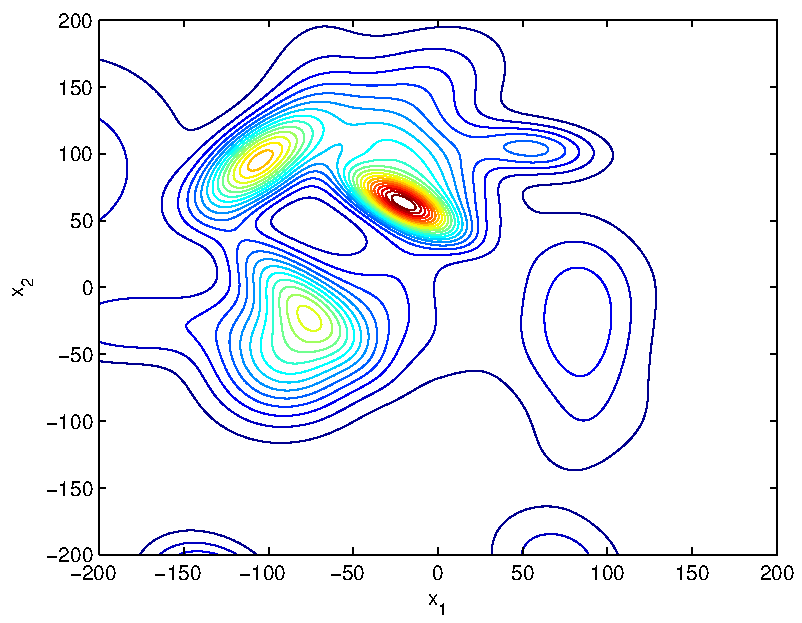
\includegraphics[width=0.7\columnwidth]{drone_terrain_map.pdf}
\caption{Contour plot of an example simulated terrain map.}
\label{fig:drone_terrain_map}
\end{figure}

\subsection{Results}

The accurate measurements of range, range rate and height constrain the region of high posterior probability to lie on a $3$ dimensional subspace, which can take some unusual shapes (see figure~\ref{fig:drone_example_frame}). This means that particle filters using simple Gaussian importance densities do not perform well --- the EPF diverges completely and produces no useful results. Furthermore, the optimal Gaussian importance density method performs poorly as the maximisation procedure struggles with the narrow mode.

Figure~\ref{fig:drone_example_frame} shows the motion of the particles from the CPPF on a typical frame, and the awkward shape of the posterior mode.{\meta REPLACE THIS WITH DETERMINISTIC PARTICLES.}
%
\begin{figure}
\centering
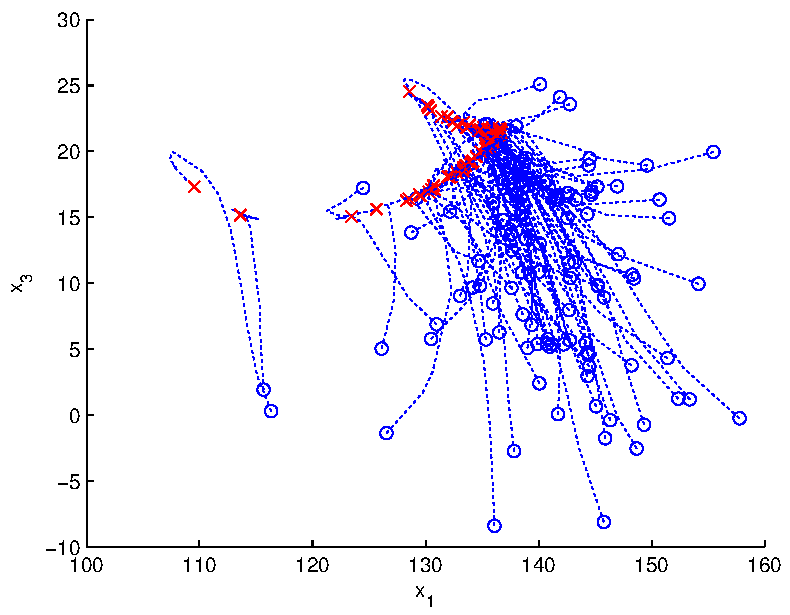
\includegraphics[width=0.7\columnwidth]{drone_example_frame.pdf}
\caption{An example of the CPPF particle motion running on the terrain tracking model, showing one horizontal and the vertical state component. Prior states are shown with circles and posterior states with crosses.}
\label{fig:drone_example_frame}
\end{figure}

Table~\ref{tab:drone_results_gaussian} shows the average ESSs and RMSEs for each algorithm over 100 simulated data sets, each of 100 time steps using the Gaussian transition density.
%
\begin{table}
\renewcommand{\arraystretch}{1.3}
\centering
\caption{Algorithm performance results on the terrain tracking model with Gaussian innovations.}
\begin{tabular}{l||c|c|c}
Algorithm                                & $N_F$ & ESS  & RMSE \\
\hline
Bootstrap                                &  6000 &  1.0 & 78.6 \\
UKF Proposal                             &   460 &  2.4 & 70.2 \\
Optimal Gaussian Proposal                &    10 &  3.1 & 62.9 \\
Deterministic Composite Proposal         &   180 & 56.4 & 22.3 \\
\end{tabular}
\label{tab:drone_results_gaussian}
\end{table}



\section{Conclusions and Extensions}

The CPPF outperforms other particle filters on complex nonlinear problems, achieving higher effective sample sizes and lower estimation errors. This improvement is achieved by using a multi-stage approximation to the optimal importance density. This comes at a higher cost in computational load, making the algorithm unsuitable for simpler models where a single-stage approximation would suffice.

Numerous extensions to the algorithm are being studied, including a generalisation of the algorithm to allow stochastic evolution of the state through pseudo-time, methods for selecting step sizes adaptively, the inclusion of MCMC steps to improve the quality of the particle population, and modifications for Gaussian mixture models.




% An example of a floating figure using the graphicx package.
% Note that \label must occur AFTER (or within) \caption.
% For figures, \caption should occur after the \includegraphics.
% Note that IEEEtran v1.7 and later has special internal code that
% is designed to preserve the operation of \label within \caption
% even when the captionsoff option is in effect. However, because
% of issues like this, it may be the safest practice to put all your
% \label just after \caption rather than within \caption{}.
%
% Reminder: the "draftcls" or "draftclsnofoot", not "draft", class
% option should be used if it is desired that the figures are to be
% displayed while in draft mode.
%
%\begin{figure}[!t]
%\centering
%\includegraphics[width=2.5in]{myfigure}
% where an .eps filename suffix will be assumed under latex,
% and a .pdf suffix will be assumed for pdflatex; or what has been declared
% via \DeclareGraphicsExtensions.
%\caption{Simulation Results}
%\label{fig_sim}
%\end{figure}

% Note that IEEE typically puts floats only at the top, even when this
% results in a large percentage of a column being occupied by floats.


% An example of a double column floating figure using two subfigures.
% (The subfig.sty package must be loaded for this to work.)
% The subfigure \label commands are set within each subfloat command, the
% \label for the overall figure must come after \caption.
% \hfil must be used as a separator to get equal spacing.
% The subfigure.sty package works much the same way, except \subfigure is
% used instead of \subfloat.
%
%\begin{figure*}[!t]
%\centerline{\subfloat[Case I]\includegraphics[width=2.5in]{subfigcase1}%
%\label{fig_first_case}}
%\hfil
%\subfloat[Case II]{\includegraphics[width=2.5in]{subfigcase2}%
%\label{fig_second_case}}}
%\caption{Simulation results}
%\label{fig_sim}
%\end{figure*}
%
% Note that often IEEE papers with subfigures do not employ subfigure
% captions (using the optional argument to \subfloat), but instead will
% reference/describe all of them (a), (b), etc., within the main caption.


% An example of a floating table. Note that, for IEEE style tables, the
% \caption command should come BEFORE the table. Table text will default to
% \footnotesize as IEEE normally uses this smaller font for tables.
% The \label must come after \caption as always.
%
%\begin{table}[!t]
%% increase table row spacing, adjust to taste
%\renewcommand{\arraystretch}{1.3}
% if using array.sty, it might be a good idea to tweak the value of
% \extrarowheight as needed to properly center the text within the cells
%\caption{An Example of a Table}
%\label{table_example}
%\centering
%% Some packages, such as MDW tools, offer better commands for making tables
%% than the plain LaTeX2e tabular which is used here.
%\begin{tabular}{|c||c|}
%\hline
%One & Two\\
%\hline
%Three & Four\\
%\hline
%\end{tabular}
%\end{table}


% Note that IEEE does not put floats in the very first column - or typically
% anywhere on the first page for that matter. Also, in-text middle ("here")
% positioning is not used. Most IEEE journals/conferences use top floats
% exclusively. Note that, LaTeX2e, unlike IEEE journals/conferences, places
% footnotes above bottom floats. This can be corrected via the \fnbelowfloat
% command of the stfloats package.




% trigger a \newpage just before the given reference
% number - used to balance the columns on the last page
% adjust value as needed - may need to be readjusted if
% the document is modified later
%\IEEEtriggeratref{8}
% The "triggered" command can be changed if desired:
%\IEEEtriggercmd{\enlargethispage{-5in}}

\bibliographystyle{IEEEtran}
%\bibliography{D:/pb404/Dropbox/PhD/OTbib}
\bibliography{C:/Personal/Peter/Dropbox/PhD/OTbib}

\end{document}


